% !TEX encoding = UTF-8 Unicode
\subsection{Fase AD: Analisi al Dettaglio}
\textbf{Periodo: dal 16/02/2015 al 22/02/2015}
\\
Questa fase comincia al termine della Fase A di Analisi dei Requisiti. È caratterizzata da una nuova analisi di tutti i documenti redatti nella fase precedente e dalla correzione di questi in base alle richieste e segnalazioni del proponente. Gli analisti provvedono all'individuazione dei nuovi requisiti, la correzione dei requisiti segnalati e si provvede all'incremento di tutti gli altri documenti.
\subsubsection{Diagramma di Gantt delle attività}
\begin{center}
	\begin{figure}[here]\centering
		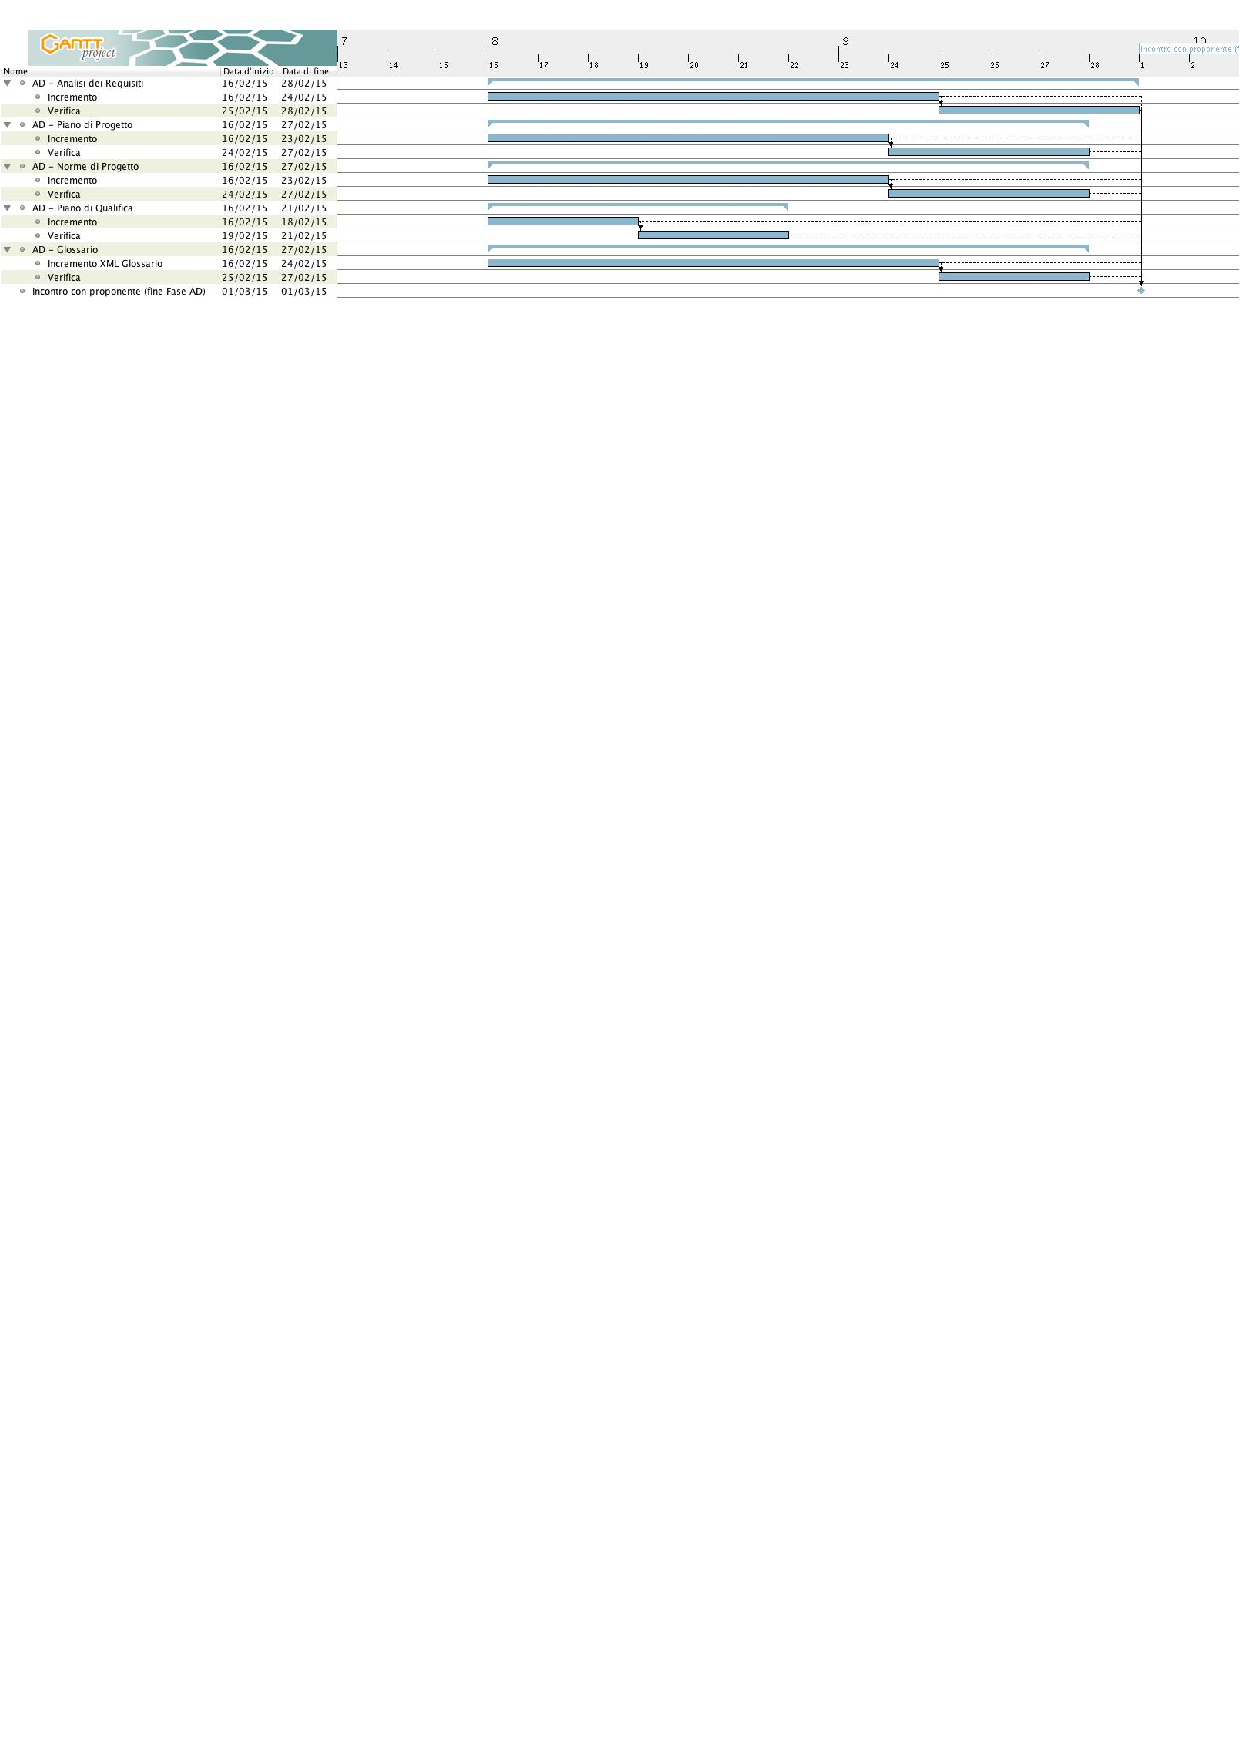
\includegraphics[width=\textwidth]{PianoDiProgetto/Pics/FaseAD}
		\caption{Gantt Fase AD}
	\end{figure}
\end{center}